\section{Interfaccia di monitoraggio}
Durante lo sviluppo del progetto è stato sviluppato in parallelo un semplice \emph{sistema di monitoring} informazioni riguardo le simulazioni eseguite ed i server Slave collegati. In particolare è stato utilizzato il linguaggio \emph{TypeScript}, con il framework \emph{Angular}. Vengono utilizati i dati forniti dalla \emph{REST API} implementata all'interno dell'esempio di avvio del progetto del server Master.

Il codice del frontend è contenuto all'interno di una apposita repository di GitHub\footnote{\url{https://github.com/ZamponiMarco/sibilla-frontend}}. Per avviare il progetto bisogna eseguire il \emph{clone della repository} ed eseguire il comando \texttt{ng serve} all'interno della cartella di root del progetto. Il frontend richiede che \emph{node.js} e il pacchetto npm \emph{@angular-cli} siano installati nel sistema.

\begin{figure}[H]
    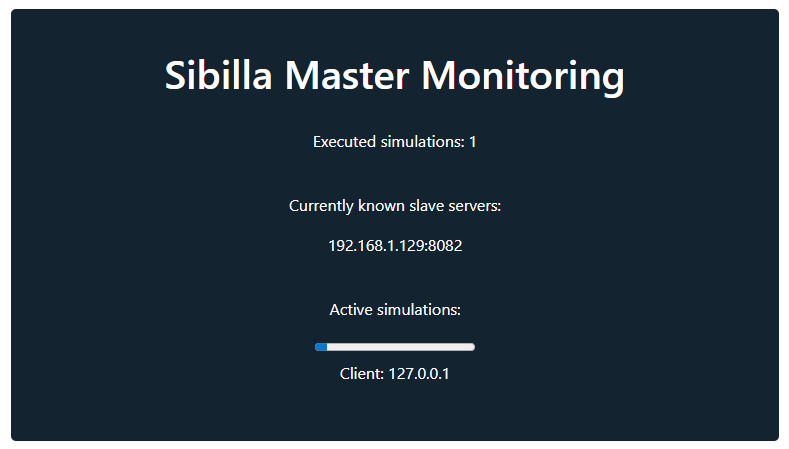
\includegraphics[width=\linewidth]{images/monitoring_frontend.PNG}
    \captionsetup{justification=centering}
    \caption{Una schermata del frontend che monitora un Master server}
\end{figure}